\chapter{RF::Cyscore: binding affinity prediction}
\label{rfcyscore}

\section{Abstract}

State-of-the-art protein-ligand docking methods are generally constrained by the traditionally low accuracy of their scoring functions, which are for binding affinity prediction and thus vital for discriminating between active and inactive compounds. Despite intensive research over the years, classical scoring functions have reached a plateau in their predictive performance. They assume a predetermined additive functional form for some sophisticated numerical features, and use standard multivariate linear regression (MLR) on experimental data to derive the coefficients.

In this study we show that such a simple functional form is detrimental for the predictive performance of a scoring function, and replacing linear regression by machine learning techniques like random forest (RF) can improve predictive performance. We investigated the conditions of applying RF under various contexts and found that given sufficient training samples RF managed to comprehensively capture the non-linearity between structural features and measured binding affinities. Incorporating more structural features and training with more samples could both boost RF performance. In addition, we analyzed the importance of structural features to binding affinity prediction using the RF variable importance tool. Lastly, we used Cyscore, a top performing empirical scoring function, as a baseline for comparison study.

In conclusion, machine-learning scoring functions are fundamentally different from classical scoring functions because the former circumvents the fixed functional form relating structural features with binding affinities. RF, but not MLR, can effectively exploit more structural features and more training samples, leading to higher predictive performance. The future availability of more X-ray crystal structures will further widen the performance gap between RF-based and MLR-based scoring functions. This further stresses the importance of substituting RF for MLR in scoring function development.

This was a collaborative project with Pedro J. Ballester from Cancer Research Center of Marseille, Marseille, France. It was published in \textit{BMC Bioinformatics} on 27 August 2014 \citep{1432}. Notably, this article has been tagged ``Highly accessed" by the journal, indicating that it may be of broad interest in the community.

\section{Background}

Protein-ligand docking is a computational tool that predicts how a ligand binds to a target protein and their binding affinity. Therefore docking is useful in elucidating intermolecular interactions and enhancing the potency and selectivity of binding in subsequent phases of the modern drug design process. Docking has a wide variety of pragmatic and successful applications in structure-based virtual screening \citep{1383}, drug repurposing \citep{1384}, lead compound optimization \citep{1385}, protein cavity identification \citep{1217}, and protein function prediction \citep{1386}.

Docking performs two main operations: predicting the position, orientation and conformation of a ligand when docked to the protein's binding site, and predicting the binding strength. The former operation is known as pose generation and the latter is known as scoring. State-of-the-art docking tools, AutoDock Vina \citep{595} and idock \citep{1153} for instance, work reasonably well at pose generation with a redocking success rate of over 50\% \citep{1362} on the benchmarks of both PDBbind v2012 and v2011 \citep{529,530} and the CSAR NRC HiQ Set 24Sept2010 \citep{857,960}. Nonetheless, the single most critical limitation of docking is the traditionally low accuracy of the scoring functions.

Classical scoring functions are defined by using an assumed, fixed functional form for the relationship between the numerical features that characterize the protein-ligand complex and its predicted binding affinity. This functional form consists of the energetic contributions of various intermolecular interactions, and is often additive. The overall binding affinity is calculated as a weighted sum of some physically meaningful terms, whereas their coefficients are typically derived from standard multivariate linear regression (MLR) on experimental data.

Cyscore \citep{1372}, a recently published empirical scoring function, assumed that the overall protein-ligand binding free energy can be divided into four terms: hydrophobic free energy, van der Waals interaction energy, hydrogen bond interaction energy and ligand's conformational entropy. Cyscore improved the prediction of hydrophobic free energy using a novel curvature-dependent surface-area model, which was claimed to be able to distinguish convex, planar and concave surface in the calculation of hydrophobic free energy.

A recent study on a congeneric series of thrombin inhibitors concluded that free energy contributions to ligand binding at the molecular level are non-additive \citep{1416}, therefore the modelling assumption of additivity models is error prone. Recent years have seen a growing number of new developments of machine-learning scoring functions, with RF-Score \citep{564} being the first that introduced a large improvement over classical approaches. RF-Score, as its name suggests, uses Random Forest (RF) \citep{1309} to implicitly learn the functional form in an completely data-driven manner, and thus circumvents the modelling assumption imposed by previous scoring functions. RF-Score was shown to significantly outperform 16 classical scoring functions when evaluated on the commonly-used PDBbind v2007 benchmark \citep{564}. Despite being a recent development, RF-Score has already been successfully used to discover a large number of innovative binders against antibacterial DHQase2 targets \citep{1281}. For the purpose of prospective virtual screening, RF-Score-v3 has now been incorporated into istar \citep{1362}, our large-scale online docking service available at http://istar.cse.cuhk.edu.hk/idock. A number of subsequent machine-learning scoring functions have also shown large improvements over classical approaches. These include, but are not limited to, NNScore 2.0 \citep{977}, SVR-KB and SVR-EP \citep{963}, CScore \citep{1194}, SVR-Score \citep{1295}, B2Bscore \citep{1410}, SFCscoreRF \citep{1347}, and ID-Score \citep{1305}.

\section{Motivation}

Despite the superior performance of RF-Score, its generalization power has not yet been evaluated under standard cross validation and leave-cluster-out cross validation \citep{774}. It would be interesting to see if substituting RF for MLR can improve the predictive performance of a classical scoring function with a fixed functional form.

\section{Objective}

In this study we compare the predictive performance of two regression models MLR and RF when trained with varying numbers of structural features and training samples, and investigate their application conditions and interpretability in various contexts. We use Cyscore as a baseline.

\section{Methods}

The following subsections introduce MLR and RF, three sets of features, three benchmarks, two types of cross validations, and four performance metrics.

\subsection{Multiple Linear Regression (MLR) with Cyscore features}

Cyscore is an empirical scoring function in an additive functional form of four energetic terms: hydrophobic free energy $\Delta G_{hydrophobic}$, van der Waals interaction energy $\Delta G_{vdw}$, hydrogen bond interaction energy $\Delta G_{hbond}$ and ligand's conformational entropy $\Delta G_{entropy}$ (equation \eqref{rfcyscore:cyscore}). Their coefficients $k_h$, $k_v$, $k_b$ and $k_e$ and the intercept $C$ were obtained by MLR on 247 high-quality complexes carefully selected from PDBbind v2012 refined set. The intercept value was not reported in the original publication, but was included in this study as usual \citep{1313} in order to quickly estimate the absolute binding affinity value, which is the ultimate goal in some real-life applications.

\begin{equation}
\Delta G_{bind} = k_h\Delta G_{hydrophobic} + k_v\Delta G_{vdw} + k_b\Delta G_{hbond} + k_e\Delta G_{entropy} + C
\label{rfcyscore:cyscore}
\end{equation}

We use MLR::Cyscore to denote the scoring function built with MLR and the 4 features from Cyscore. It is noteworthy that Cyscore is a sheer MLR model, unlike AutoDock Vina \citep{595} which is a quasi MLR model because the number of rotatable bonds $N_{rot}$ is in the denominator in order to penalize ligand flexibility (see \citep{1362} for the exact equation) and therefore MLR::Vina would require an additional grid search for the weight of the $N_{rot}$ parameter. Hence this study allows a more direct comparison between MLR and RF.

\subsection{Random Forest (RF) with Cyscore, AutoDock Vina and RF-Score features}

A RF \citep{1309} is a consensus of a large number of different decision trees generated from random bootstrap sampling of the same training data. During tree construction, at each inner node RF chooses the best splitting feature that results in the highest purity gain from a normally small number (mtry) of randomly selected features instead of utilizing all input features. In the case of regression, the final output is computed as the arithmetic mean of all individual tree predictions in the RF. More details on RF construction can be found in \citep{564,1362}.

In this study, multiple RFs of the default number of 500 trees were built using values of the mtry control parameter from one to the total number of input features. The selected RF was the one that resulted in the lowest root mean square error (RMSE) on the Out-of-Bag (OOB) samples of the training set. We used just one single random seed for training because seed is not a significant impact factor of the predictive performance. Using fewer seeds also has the advantage of computationally faster training process.

In our experiments we aimed at analyzing how RF responds to varying numbers of features. So we selected three sets of features: Cyscore \citep{1372}, AutoDock Vina \citep{595} and RF-Score \citep{564}. Cyscore comprises four numerical features: $\Delta G_{hydrophobic}$, $\Delta G_{vdw}$, $\Delta G_{hbond}$ and $\Delta G_{entropy}$. AutoDock Vina comprises six numerical features: $Gauss_1$, $Gauss_2$, $Repulsion$, $Hydrophobic$, $HBonding$ and $N_{rot}$. RF-Score comprises 36 features, defined as the number of intermolecular contacts between two elemental atom types. Four atom types for proteins (C, N, O, S) and nine for ligands (C, N, O, S, P, F, Cl, Br, I) were selected so as to produce a dense set of features while considering all the heavy atom types commonly observed in protein-ligand complexes. Table \ref{rfcyscore:features} summarizes the three combinations of these feature sets used to train RF models. Totally four models, MLR::Cyscore, RF::Cyscore, RF::CyscoreVina and RF::CyscoreVinaElem, were evaluated in this study.

\begin{table}
\caption{The three combinations of three different sets of features used to train RF models.}
\label{rfcyscore:features}
\begin{tabular}{ll}
\hline
model & features\\
\hline
RF::Cyscore         & 4 Cyscore features\\
RF::CyscoreVina     & 4 Cyscore features + 6 AutoDock Vina features\\
RF::CyscoreVinaElem & 4 Cyscore features + 6 AutoDock Vina features + 36 RF-Score features\\
\hline
\end{tabular}
\end{table}

\subsection{PDBbind v2007 and v2012 benchmarks}

The PDBbind \citep{529,530} benchmark is arguably the most widely used for binding affinity prediction. It is a diverse collection of experimentally resolved protein-ligand complexes, assembled through a systematic mining of the yearly releases of the entire PDB (Protein Data Bank) \citep{540,537}. For each complex, the experimentally measured binding affinity, in terms of either dissociation constant Kd or inhibition constant Ki, was manually collected from its primary literature reference. The complexes with a resolution of $\le$2.5\AA\ and with the ligand comprising only nine common heavy atom types (C, N, O, F, P, S, Cl, Br, I) were filtered to constitute the refined set. These complexes were then clustered by protein sequence identity with a cutoff of 90\%, and for each of the resulting clusters with at least five complexes, the three complexes with the highest, median and lowest binding affinity were selected to constitute the core set. Due to the structural diversity of the core set, it is a common practice to use the core set as a test set and the remaining complexes in the refined set as a training set.

Cyscore was tested on two independent sets: PDBbind v2007 core set (N=195) and PDBbind v2012 core set (N=201), whose experimental binding affinities span 12.56 and 9.85 pKd units, respectively. Cyscore was trained on a special set of 247 complexes carefully selected from the PDBbind v2012 refined set using certain criteria \citep{1372} (e.g. structural resolution \textless\ 1.8\AA, binding affinity spans 1 to 11 kcal/mol, protein sequence similarity and ligand chemical composition are different from the test set), ensuring that the training complexes are of high quality and do not overlap with any of the two test sets. In this study in order to make a fair comparison to Cyscore we used exactly the same training and test sets.

Moreover, in view of the fact that 16 classical scoring functions have already been evaluated \citep{1313} on PDBbind v2007 core set and the top performing of them (e.g. X-Score \citep{573}) were trained on the remaining 1105 complexes in PDBbind v2007 refined set, we also used these 1105 complexes to constitute another training set to permit a direct comparison. Using predefined training and test sets, where other scoring functions had previously been trained and tested, has the advantage of reducing the risk of using a benchmark complementary to one particular scoring function.

Similarly for the PDBbind v2012 benchmark, we used an extra training set comprising the complexes in PDBbind v2012 refined set excluding those in PDBbind v2012 core set. This led to a total of 2696 complexes. By construction, this training set does not overlap with the test set.

\subsection{PDBbind v2013 round-robin benchmark}

We propose a new benchmark with the purpose to investigate how predictive performance of the four models changes in cross validation and with different numbers of training samples. We used PDBbind v2013 refined set (N=2959), which was the latest version at the time of writing and constituted the most comprehensive and publicly available structural dataset suitable for training scoring functions.

We used 5-fold cross validation, as was used by the recently published empirical scoring function ID-Score \citep{1305}, to estimate overfitting and thus generalization errors. The entire PDBbind v2013 refined set (N=2959) was decomposed into five equal partitions using uniform sampling on a round-robin basis: the entire 2959 complexes were first sorted in the ascending order of their measured binding affinity, and the complexes with the 1st, 6th, 11th, etc. lowest binding affinity belonged to the first partition, the complexes with the 2nd, 7th, 12th, etc. lowest binding affinity belonged to the second partition, and so on. This partitioning method, though not entirely random, has two advantages. On one hand, each partition is guaranteed to span the largest range of binding affinities and incorporates the largest structural diversity of different protein families. On the other hand, each partition is composed of a deterministic list of complexes, permitting reproducibility and comparisons in future studies. Table \ref{rfcyscore:partitions} summarizes the statistics of the five partitions. Figure \ref{rfcyscore:cv} plots the binding affinity distribution of pKd values of the five partitions.

\begin{table}
\caption{Statistics of the five partitions of PDBbind v2013 refined set.}
\label{rfcyscore:partitions}
\begin{tabular}{rrrr}
\hline
\# & complexes & lowest pKd & highest pKd\\
\hline
1 & 592 & 2.00 & 11.74\\
2 & 592 & 2.00 & 11.80\\
3 & 592 & 2.00 & 11.85\\
4 & 592 & 2.00 & 11.92\\
5 & 591 & 2.05 & 11.72\\
\hline
\end{tabular}
\end{table}

\begin{figure}
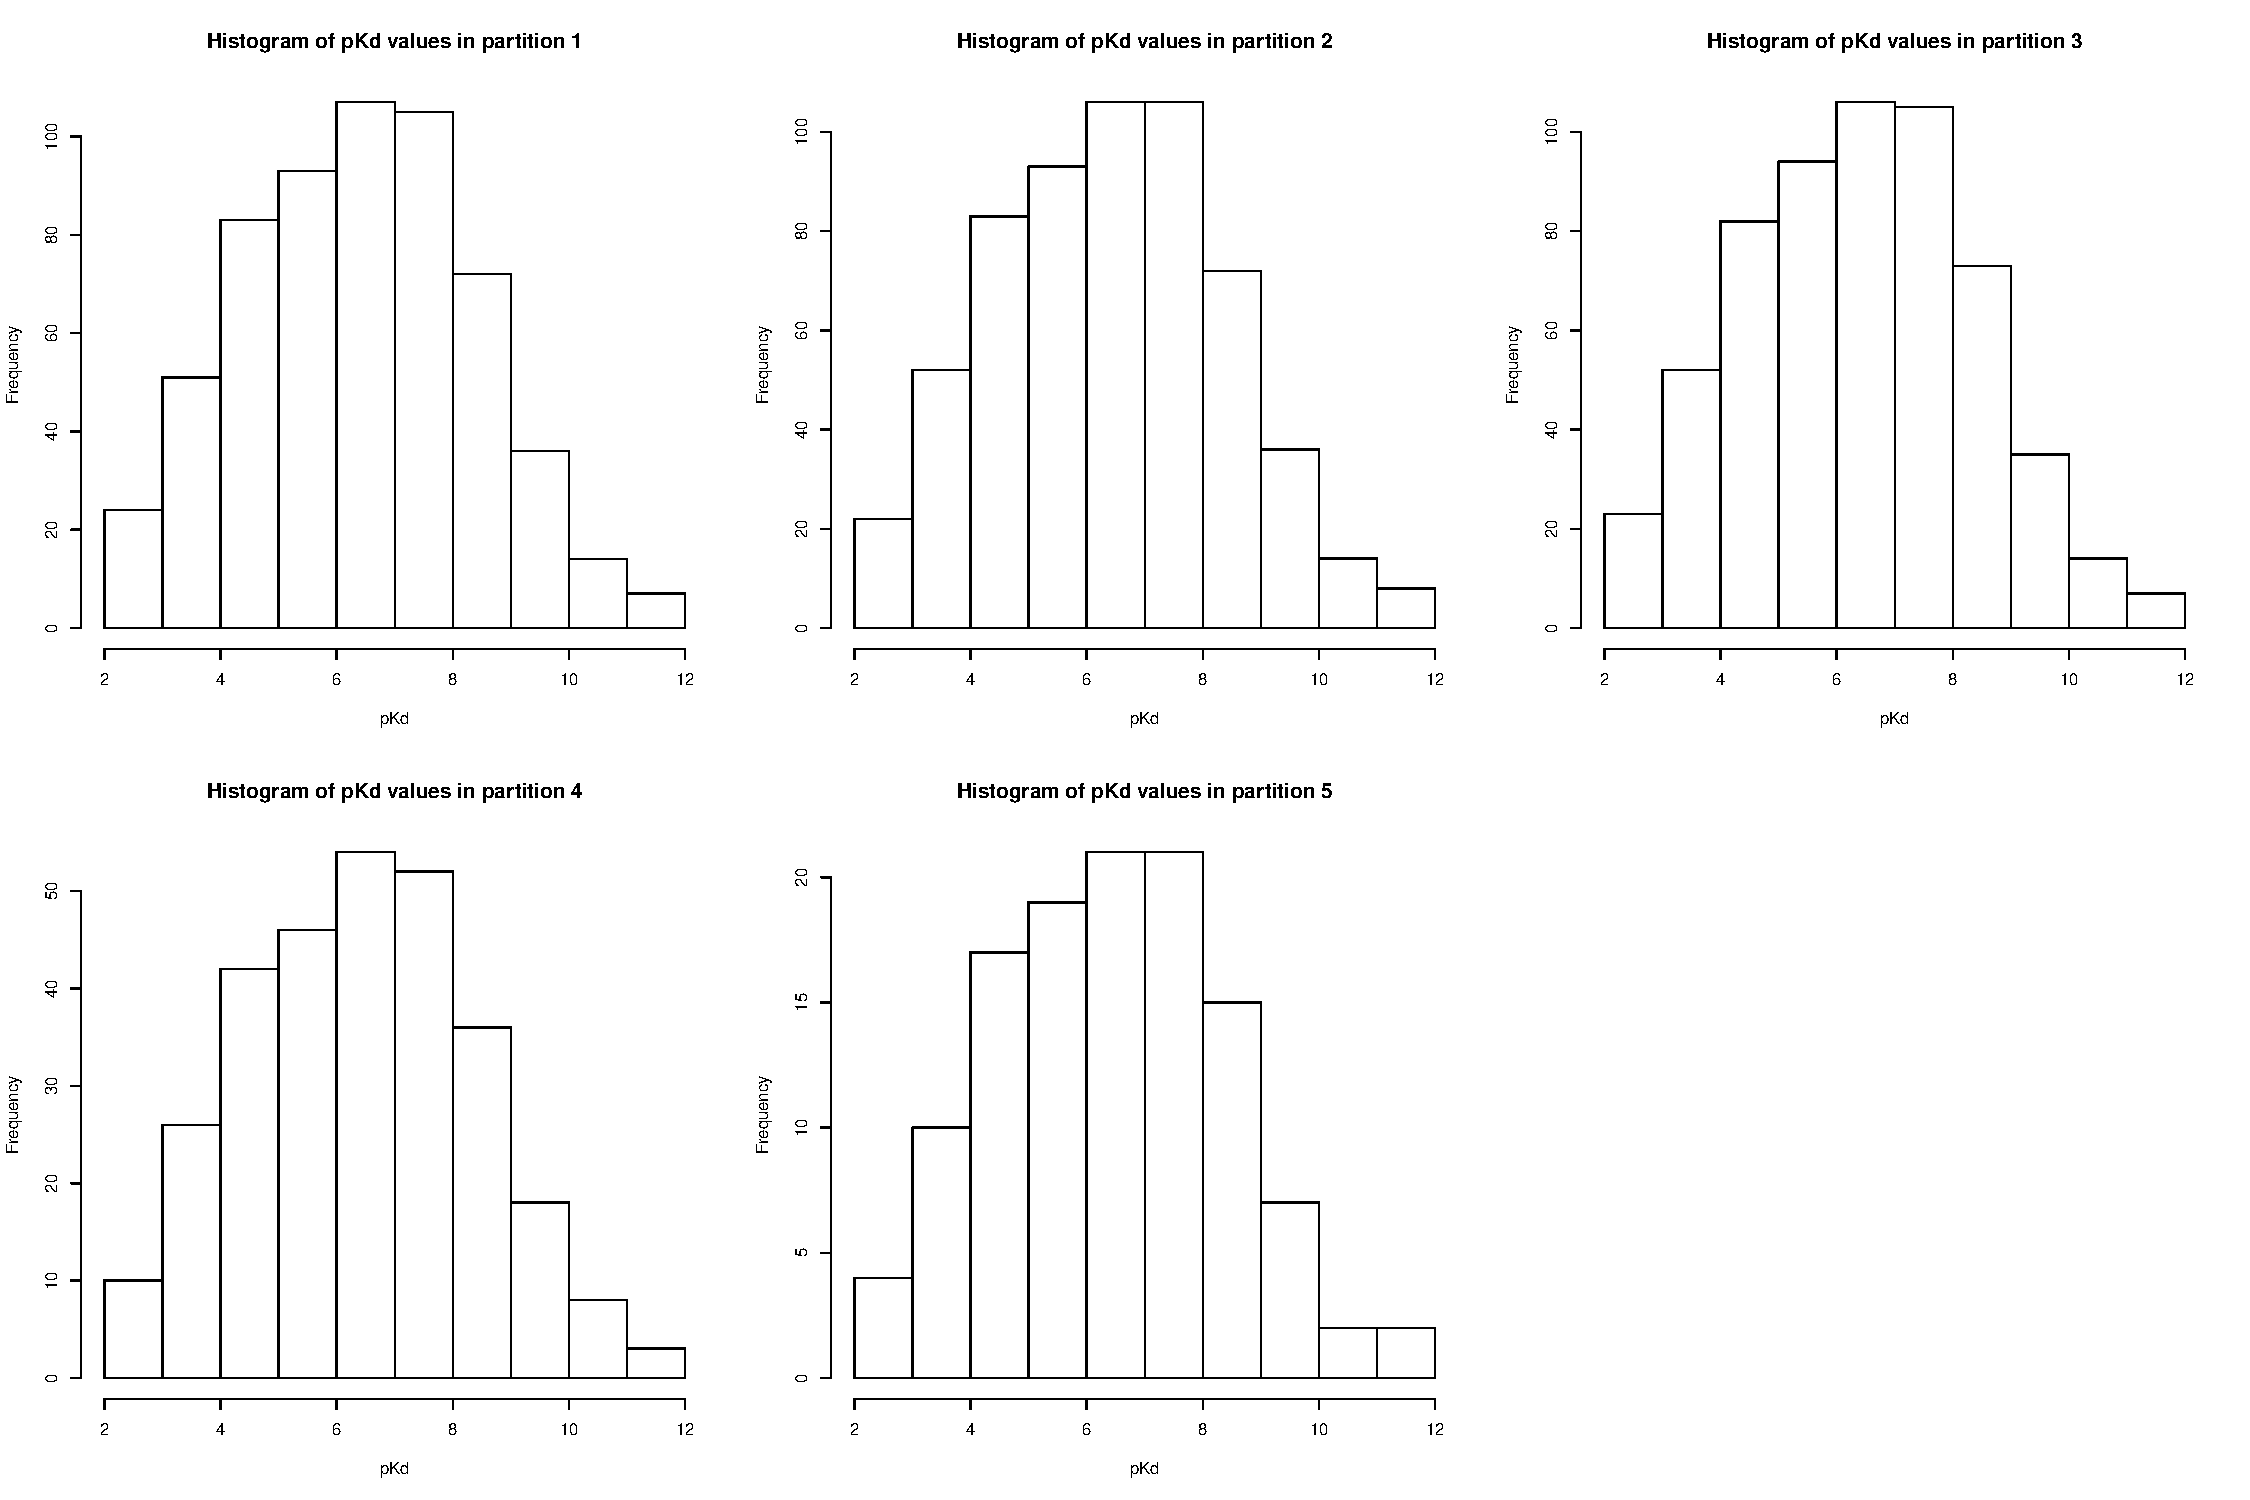
\includegraphics[width=\linewidth]{../rfcyscore/cv.pdf}
\caption{Histograms of pKd values of the five partitions of PDBbind v2013 refined set.}
\label{rfcyscore:cv}
\end{figure}

We then used the partition on which the optimal performance was obtained (It turned out to be partition 2 (N=592). See the Results section below.) as the test set in PDBbind v2013 round-robin benchmark, and used the remaining four partitions (1, 3, 4, 5) to construct four training sets of incremental sizes: the first training set comprises partition 1 (N=592), the second training set comprises partitions 1 and 3 (N=1184), the third training set comprises partitions 1, 3 and 4 (N=1776), and the fourth training set comprises partitions 1, 3, 4 and 5 (N=2367). By construction, this new benchmark helps to study how predictive performance varies with training set size. Moreover, its test set has a substantially larger number of complexes (N=592) compared to PDBbind v2007 (N=195) and v2012 (N=201) benchmarks, making this new benchmark not being a redundant duplication of the previous two benchmarks. Table \ref{rfcyscore:benchmarks} summarizes the numbers of test and training samples for the three benchmarks.

\begin{table}
\caption{The numbers of test samples and training samples for the PDBbind v2007, v2012 and v2013 benchmarks.}
\label{rfcyscore:benchmarks}
\begin{tabular}{ccc}
\hline
benchmark & test samples & training samples\\
\hline
v2007 & 195 & 247, 1105\\
v2012 & 201 & 247, 2696\\
v2013 & 592 & 592, 1184, 1776, 2367\\
\hline
\end{tabular}
\end{table}

\subsection{Leave-cluster-out cross validation (LCOCV)}

Leave-cluster-out cross validation (LCOCV) \citep{774}, in contrast to standard cross validation, divides the whole set of complexes into protein families instead of random subsets. Each protein family, or each cluster, is typically determined by 90\% protein sequence identity. A total of 23 selected protein families with at least ten complexes are treated as individual clusters, labeled as A to W. Protein families with four to nine complexes are combined into cluster X. Protein families with two to three complexes are combined into cluster Y. Singletons are combined into cluster Z. Each cluster is iteratively left out of the training set and used to evaluate the predictive performance of the scoring function. The performance on each cluster can be inspected individually, and the overall performance can be estimated by averaging over all clusters.

So far LCOCV has been applied to the assessment of six scoring functions, which are RF-Score \citep{774,1194,1410}, ddPLAT+MOE \citep{1414}, CScore \citep{1194}, B2Bscore \citep{1410}, SFCscoreRF \citep{1347} and the work of Ross et al. \citep{1415}. The first four scoring functions were evaluated on PDBbind v2009 refined set, while SFCscoreRF was on PDBbind v2010 refined set and the work of Ross et al. was on PDBbind v2011 refined set. For the purpose of comparison to these scoring functions, we used PDBbind v2009 refined set (N=1741) to perform LCOCV. We discarded the 1xr8 entry in cluster X because its ligand is far away from its protein, thereby leaving 1740 complexes. Figure \ref{rfcyscore:lcocv} plots the binding affinity distribution of pKd values of the 26 clusters.

\begin{figure}
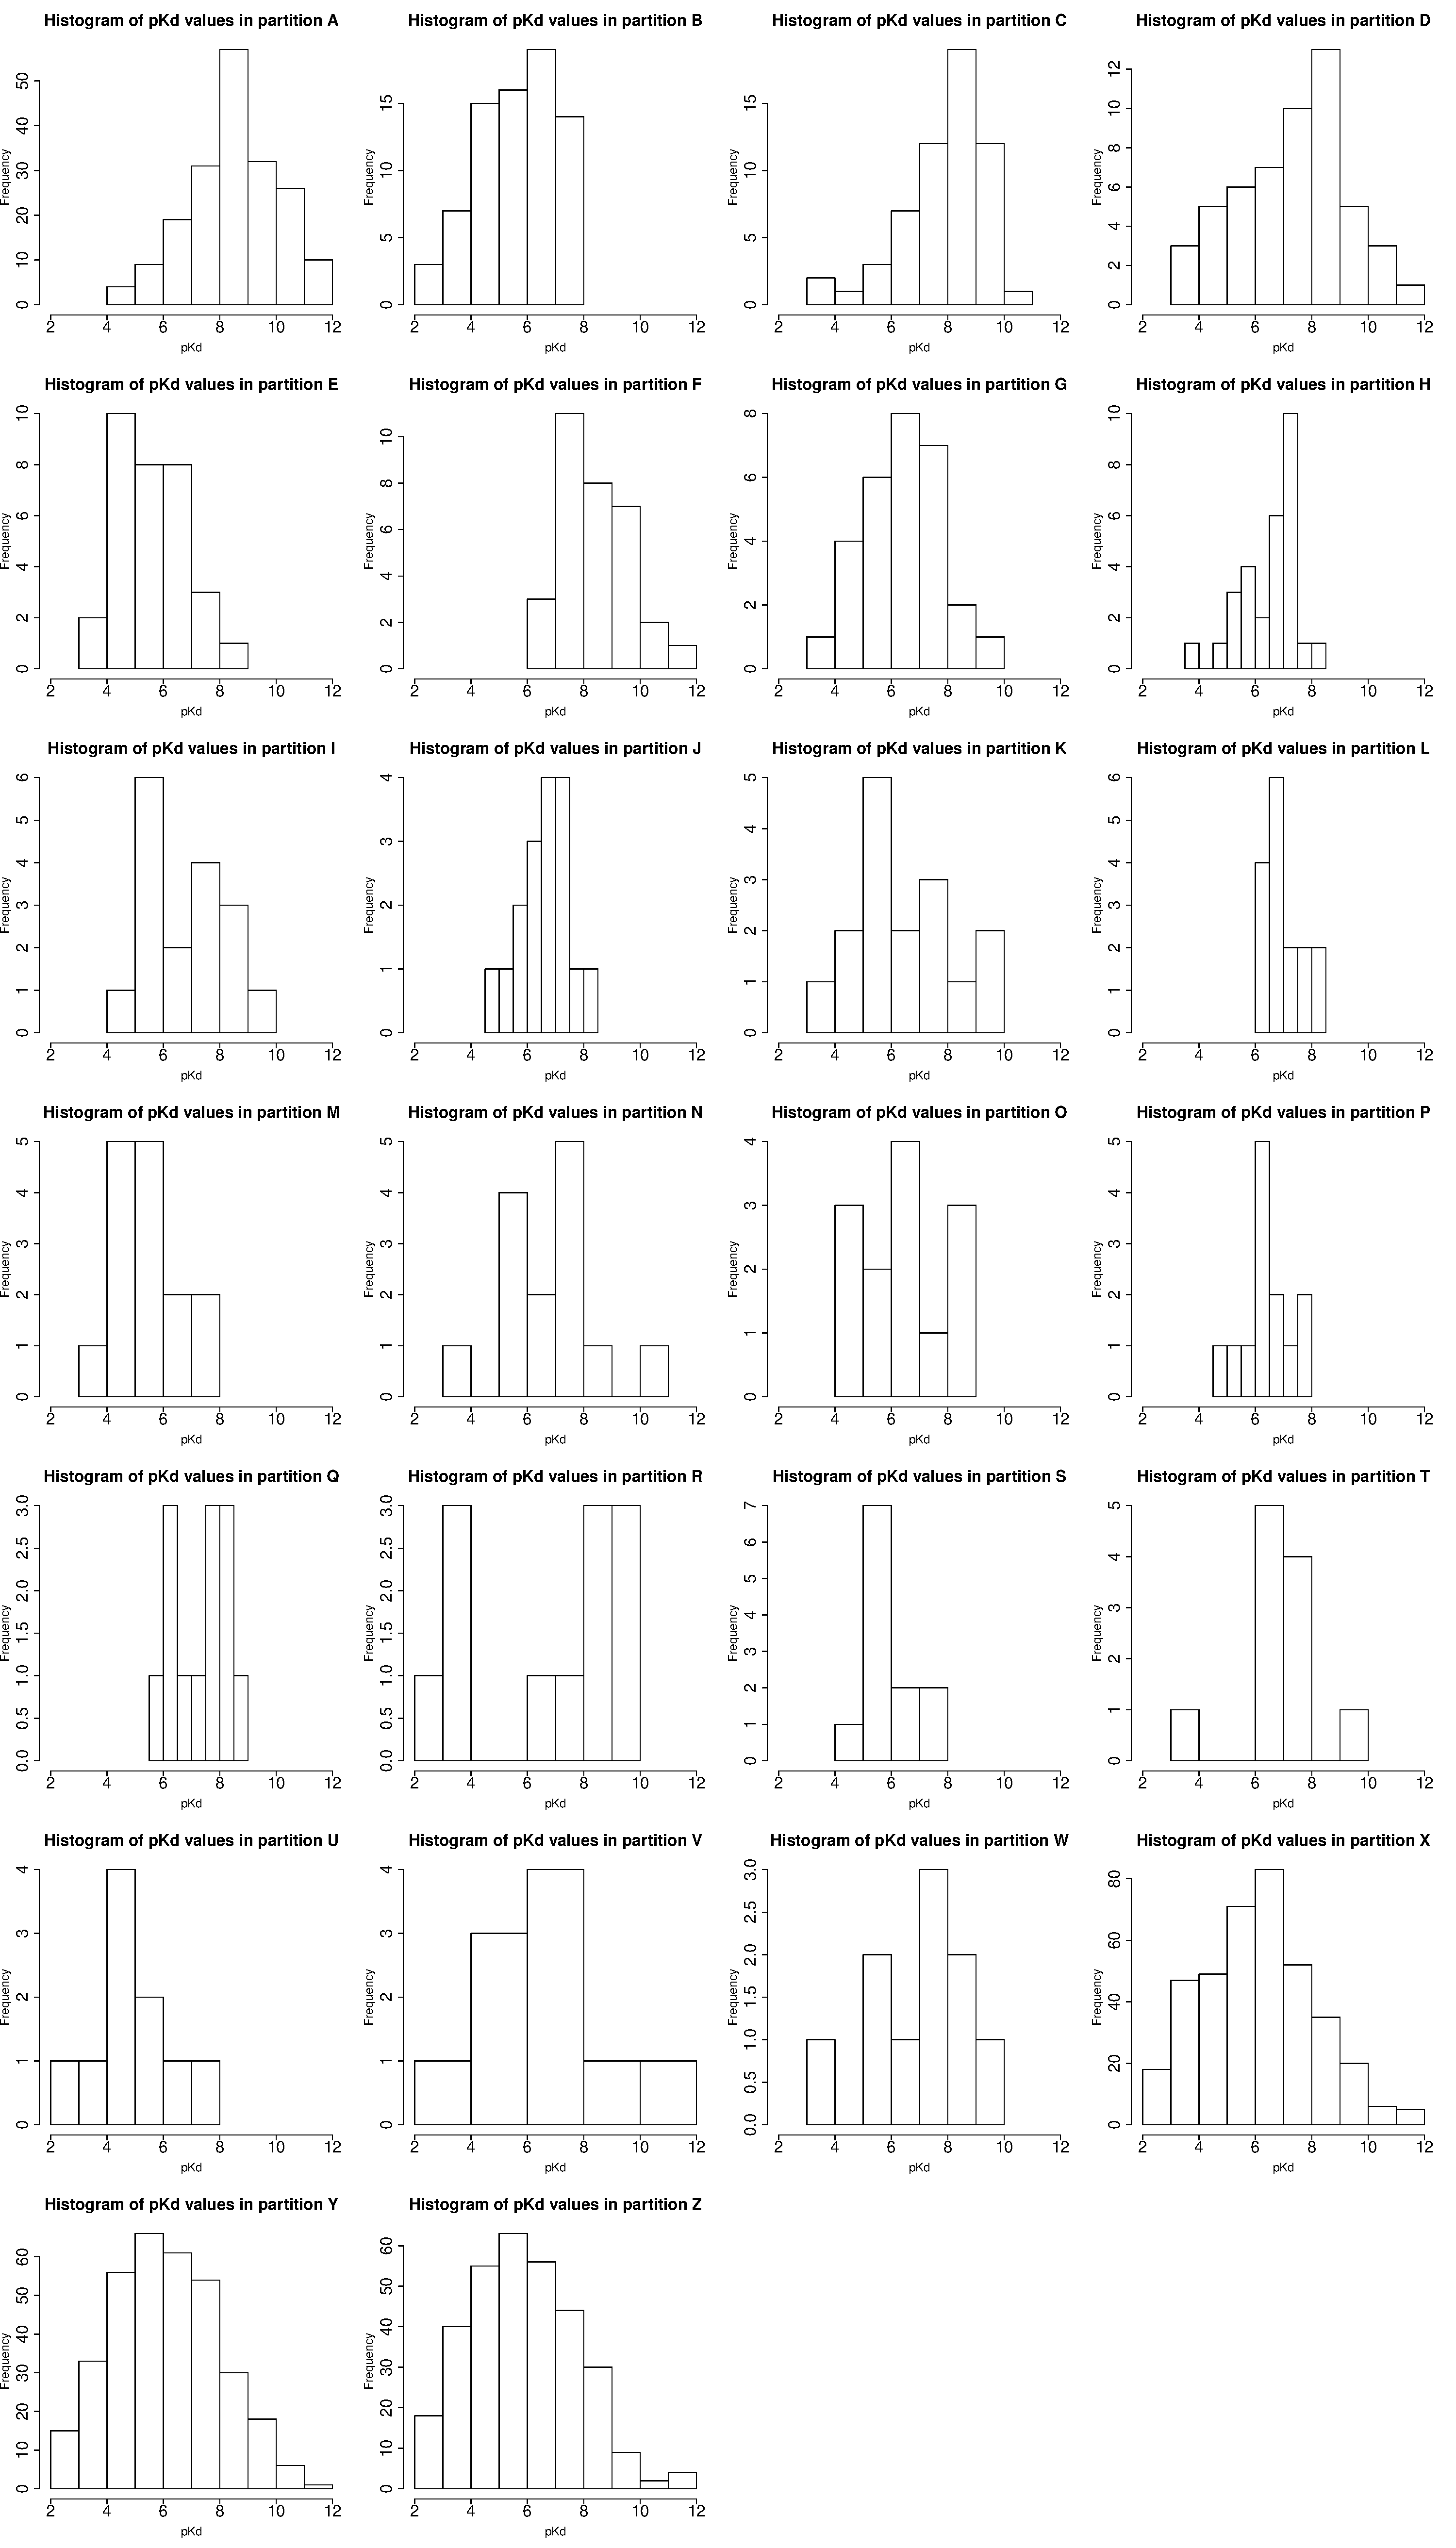
\includegraphics[width=\linewidth]{../rfcyscore/lcocv.pdf}
\caption{Histograms of pKd values of the 26 clusters of PDBbind v2009 refined set.}
\label{rfcyscore:lcocv}
\end{figure}

\subsection{Performance metrics}

Predictive performance was quantified through standard deviation SD in linear correlation, Pearson correlation coefficient Rp and Spearman correlation coefficient Rs between the measured and predicted binding affinities of the test set. These metrics are commonly used in the community \citep{1313}. The SD metric is essentially the residual standard error (RSE) metric used in some other studies \citep{963}. The above three metrics are invariant under linear transformations. Changing the intercept or coefficient values in equation \eqref{rfcyscore:cyscore} affects none of these metrics. So they are mainly for comparative purpose. In some applications, however, the ultimate goal of scoring functions is to predict an absolute binding affinity value as close to the measured value as possible. Therefore we use a more realistic metric, the root mean square error RMSE between measured and predicted binding affinities without coupling a linear correlation. Lower values in RMSE and SD and higher values in Rp and Rs indicate better predictive performance.

Mathematically, equations \eqref{rfcyscore:rmse}, \eqref{rfcyscore:sdev}, \eqref{rfcyscore:pcor} and \eqref{rfcyscore:scor} show the expressions of the four metrics. Given a scoring function $f$ and the features $\mathbf{x}_i$ characterizing the $i$th complex out of $n$ complexes in the test set, $p_i=f(\mathbf{x}_i)$ is the predicted binding affinity, $\{\hat{p}_i\}_{i=1}^n$ are the fitted values from the linear model between $\{y_i\}_{i=1}^n$ and $\{p_i\}_{i=1}^n$ on the test set, whereas $\{y^r_i\}_{i=1}^n$ and $\{p^r_i\}_{i=1}^n$ are the rankings of $\{y_i\}_{i=1}^n$ and $\{p_i\}_{i=1}^n$, respectively.

\begin{equation}
RMSE=\sqrt{\frac{1}{n}\sum_{i=1}^n(p_i-y_i)^2}
\label{rfcyscore:rmse}
\end{equation}

\begin{equation}
SD=\sqrt{\frac{1}{n-2}\sum_{i=1}^n(\hat{p}_i-y_i)^2}
\label{rfcyscore:sdev}
\end{equation}

\begin{equation}
R_p=\frac{n\sum_{i=1}^np_iy_i-\sum_{i=1}^np_i\sum_{i=1}^ny_i}{\sqrt{(n\sum_{i=1}^n(p_i)^2-(\sum_{i=1}^np_i)^2)(n\sum_{i=1}^n(y_i)^2-(\sum_{i=1}^ny_i)^2)}}
\label{rfcyscore:pcor}
\end{equation}

\begin{equation}
R_s=\frac{n\sum_{i=1}^np^r_iy^r_i-\sum_{i=1}^np^r_i\sum_{i=1}^ny^r_i}{\sqrt{(n\sum_{i=1}^n(p^r_i)^2-(\sum_{i=1}^np^r_i)^2)(n\sum_{i=1}^n(y^r_i)^2-(\sum_{i=1}^ny^r_i)^2)}}
\label{rfcyscore:scor}
\end{equation}

\section{Results and discussion}

\subsection{MLR::Cyscore performance does not increase with more training samples}

Figure \ref{rfcyscore:stat} plots the predictive performance of MLR::Cyscore, RF::Cyscore, RF::CyscoreVina and RF::CyscoreVinaElem using different numbers of training samples. The first row is for root mean square error RMSE, the second row is for standard deviation SD in linear correlation, the third row is for Pearson correlation coefficient Rp, and the fourth row is for Spearman correlation coefficient Rs. The left column is for PDBbind v2007 benchmark (N=195), the center column is for PDBbind v2012 benchmark (N=201), and the right column is for PDBbind v2013 round-robin benchmark (N=592).

\begin{figure}
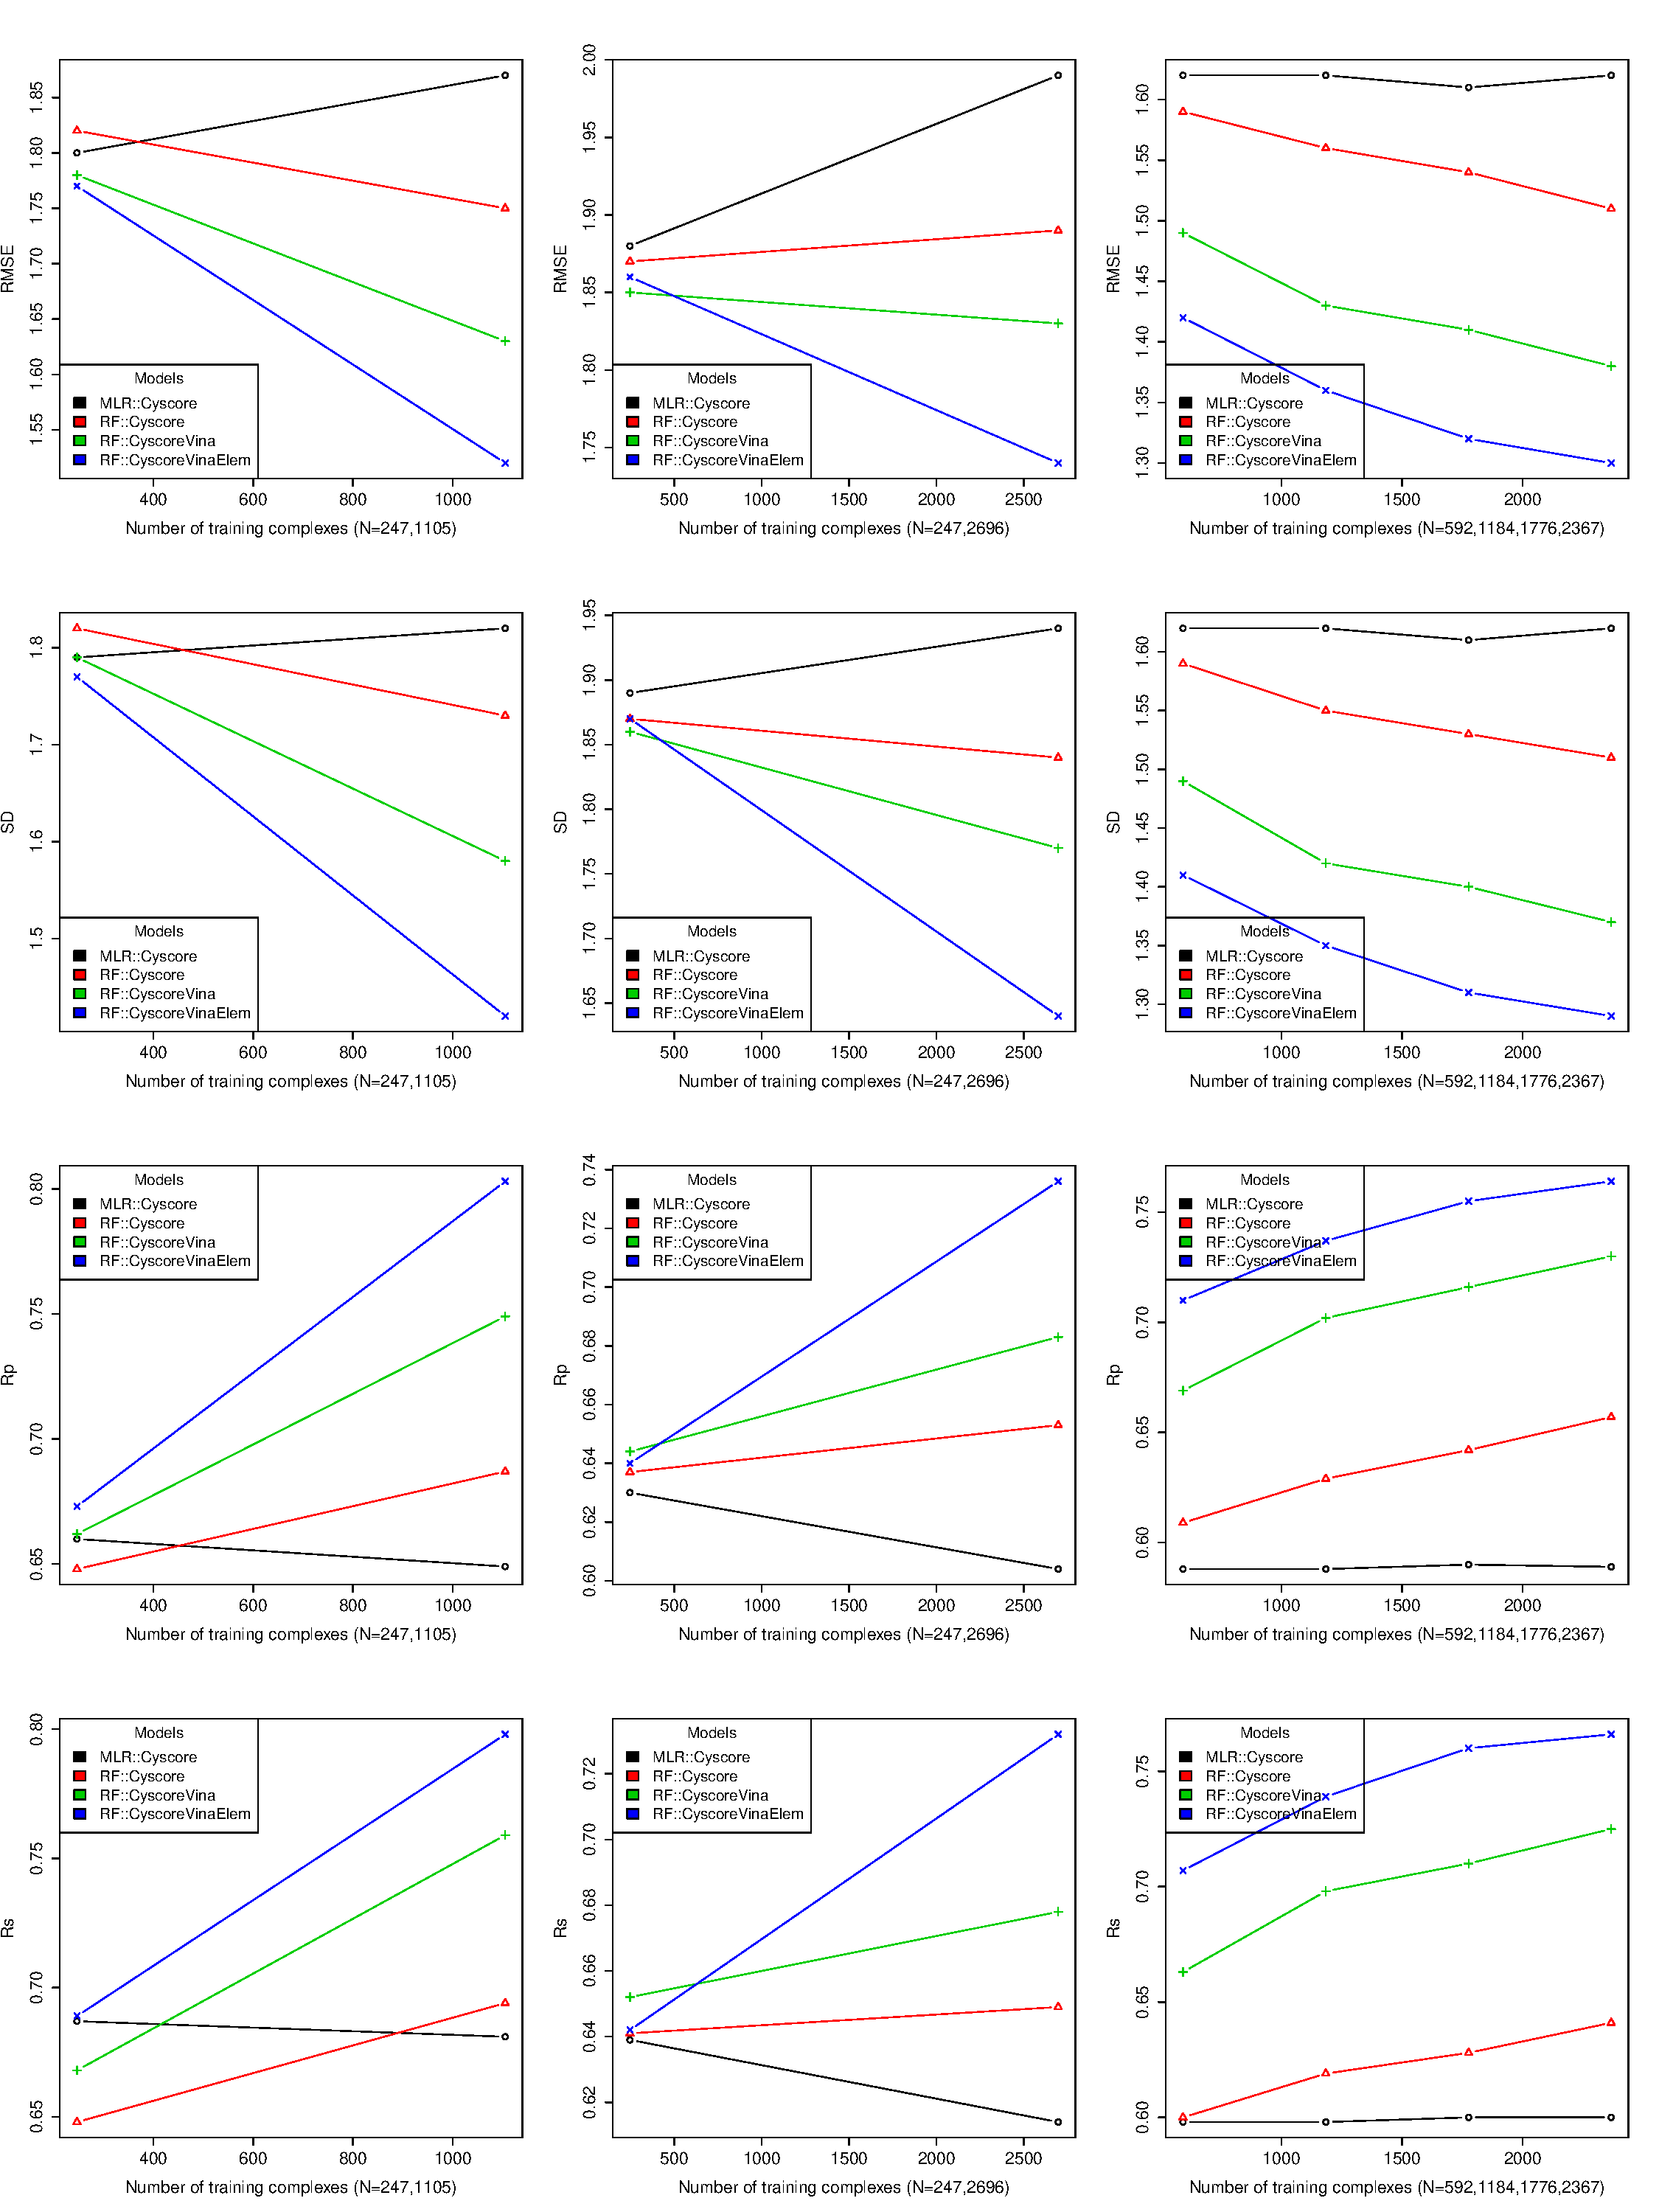
\includegraphics[width=\linewidth]{../rfcyscore/stat.pdf}
\caption{Predictive performance of MLR::Cyscore, RF::Cyscore, RF::CyscoreVina and RF::CyscoreVinaElem trained with varying numbers of samples.}
\label{rfcyscore:stat}
\end{figure}

On both PDBbind v2007 and v2012 benchmarks, MLR::Cyscore performed best when it was trained on the 247 carefully selected complexes used by Cyscore \citep{1372}. Its performance dropped when more complexes were used for training. On PDBbind v2013 round-robin benchmark, MLR::Cyscore performance stayed nearly flat regardless of training set sizes.

These results show that MLR::Cyscore cannot exploit large sets of structural data given only a small set of sophisticated features. Feeding more training samples to MLR::Cyscore actually increases the difficulty in regressing the coefficients well. Generally it would be a good idea to select the training complexes that provide the best performance on a test set, as was the case of Cyscore. But in real applications the binding affinities of the test set are not known and unfortunately selection of training complexes is not performed blindly without measuring performance on test set.

\subsection{RF performance increases with more structural features and training samples}

As seen from Figure \ref{rfcyscore:stat}, on all the three benchmarks, given the same set of features, the RF models trained with more samples resulted in higher predictive accuracy. Likewise, given the same training samples, the RF models trained with more features resulted in higher predictive accuracy.

These results suggest that RF is able to effectively exploiting a comprehensive set of structural features and training samples. Generally the more training samples, the more knowledge for RF to learn so as to capture the non-linearity of the structural data. Likewise, the more appropriate features, the higher probability of choosing the best splitting feature that can result in a high purity gain at non-leaf nodes during RF construction, and thus the higher chance of improved RF performance.

\subsection{RF models perform consistently well in cross validation}

Table \ref{rfcyscore:cv-stat} shows the results of 5-fold cross validation for all the four models on the five partitions of PDBbind v2013 refined set (N=2959). Interestingly, the four models all exhibited the best performance on partition 2. In terms of average performance, the relative ranking is consistent, where RF::CyscoreVinaElem (RMSE=1.35, SD=1.35, Rp=0.738, Rs=0.738) is better than RF::CyscoreVina (RMSE=1.44, SD=1.44, Rp=0.693, Rs=0.690), which is better than RF::Cyscore (RMSE=1.59, SD=1.59, Rp=0.603, Rs=0.587), which is better than MLR::Cyscore (RMSE=1.66, SD=1.66, Rp=0.556, Rs=0.559).

\begin{table}
\caption{Cross validation results of the four models on the five partitions of PDBbind v2013 refined set.}
\label{rfcyscore:cv-stat}
\begin{tabular}{rrrrrr}
\hline
\# & N & RMSE & SD & Rp & Rs\\
\hline
\multicolumn{6}{l}{MLR::Cyscore}\\
  1 & 592 & 1.66 & 1.66 & 0.560 & 0.555\\
  2 & 592 & 1.62 & 1.62 & 0.589 & 0.600\\
  3 & 592 & 1.69 & 1.70 & 0.531 & 0.529\\
  4 & 592 & 1.68 & 1.68 & 0.542 & 0.557\\
  5 & 591 & 1.65 & 1.65 & 0.559 & 0.553\\
avg &     & 1.66 & 1.66 & 0.556 & 0.559\\
\hline
\multicolumn{6}{l}{RF::Cyscore}\\
  1 & 592 & 1.60 & 1.60 & 0.601 & 0.588\\
  2 & 592 & 1.51 & 1.51 & 0.657 & 0.641\\
  3 & 592 & 1.66 & 1.66 & 0.561 & 0.545\\
  4 & 592 & 1.63 & 1.63 & 0.580 & 0.576\\
  5 & 591 & 1.57 & 1.57 & 0.615 & 0.586\\
avg &     & 1.59 & 1.59 & 0.603 & 0.587\\
\hline
\multicolumn{6}{l}{RF::CyscoreVina}\\
  1 & 592 & 1.41 & 1.41 & 0.708 & 0.709\\
  2 & 592 & 1.38 & 1.37 & 0.730 & 0.725\\
  3 & 592 & 1.49 & 1.49 & 0.668 & 0.665\\
  4 & 592 & 1.51 & 1.51 & 0.657 & 0.661\\
  5 & 591 & 1.42 & 1.42 & 0.701 & 0.692\\
avg &     & 1.44 & 1.44 & 0.693 & 0.690\\
\hline
\multicolumn{6}{l}{RF::CyscoreVinaElem}\\
  1 & 592 & 1.33 & 1.33 & 0.748 & 0.746\\
  2 & 592 & 1.30 & 1.29 & 0.764 & 0.766\\
  3 & 592 & 1.41 & 1.41 & 0.711 & 0.709\\
  4 & 592 & 1.41 & 1.41 & 0.711 & 0.722\\
  5 & 591 & 1.30 & 1.30 & 0.758 & 0.749\\
avg &     & 1.35 & 1.35 & 0.738 & 0.738\\
\hline
\end{tabular}
\end{table}

\subsection{Leave-cluster-out cross validation leads to unrealistically low performance}

Tables \ref{rfcyscore:lcocv1}, \ref{rfcyscore:lcocv2}, \ref{rfcyscore:lcocv3} and \ref{rfcyscore:lcocv4} show the results of leave-cluster-out cross validation (LCOCV) for all the four models on the 23 protein families (A to W) and 3 multi-family clusters (X to Z) of PDBbind v2009 refined set. Not unexpectedly, the observed performance is considerably heterogeneous across the different protein families. These results indeed agree with the LCOCV results of six other scoring functions from previous studies \citep{774,1414,1194,1410,1347,1415}. Having analyzed the LCOCV statistics of all these ten scoring functions, we found that they all performed well in certain clusters (e.g. trypsin and $\beta$-secretase I) and poorly in some other clusters (e.g. HIV protease and factor Xa). The reasons for the large spread of performance across the different clusters are manifold, and a comprehensive analysis for each protein family is beyond the scope of this study. As pointed out in \citep{1347}, eliminating all the HIV protease complexes leads to an imbalance between the training and test sets because HIV protease inhibitors are on average much larger than the ligands of the other targets. This illustrates that the LCOCV results should not be directly interpreted as performance measures on particular protein families. Moreover, the small size of many clusters and the limited range of measured binding affinity values therein render a satisfactory prediction of the ranking rather challenging.

\begin{table}
\caption{Leave-cluster-out cross validation results of MLR::Cyscore.}
\label{rfcyscore:lcocv1}
\begin{tabular}{lcrrrrr}
\hline
cluster name & cluster & N & RMSE & SD & Rp & Rs\\
\hline
HIV protease                   & A & 188 & 1.65 & 1.53 & 0.259 & 0.216\\
trypsin                        & B &  74 & 1.24 & 1.11 & 0.612 & 0.695\\
carbonic anhydrase             & C &  57 & 2.47 & 1.35 & 0.473 & 0.343\\
thrombin                       & D &  53 & 1.52 & 1.40 & 0.702 & 0.676\\
protein tyrosine phosphatase   & E &  32 & 1.23 & 1.06 & 0.411 & 0.313\\
factor Xa                      & F &  32 & 1.18 & 0.96 & 0.604 & 0.634\\
urokinase                      & G &  29 & 1.15 & 1.14 & 0.643 & 0.602\\
different similar transporters & H &  29 & 0.96 & 0.96 & 0.285 & 0.122\\
c-AMP dependent kinase         & I &  17 & 1.32 & 1.15 & 0.537 & 0.537\\
$\beta$-glucosidase            & J &  17 & 1.03 & 0.78 & 0.383 & 0.316\\
antibodies                     & K &  16 & 1.41 & 1.43 & 0.693 & 0.706\\
casein kinase II               & L &  16 & 0.75 & 0.58 & 0.538 & 0.358\\
ribonuclease                   & M &  15 & 1.12 & 1.20 & 0.230 & 0.340\\
thermolysin                    & N &  14 & 1.15 & 1.14 & 0.680 & 0.635\\
CDK2 kinase                    & O &  13 & 1.06 & 0.80 & 0.841 & 0.812\\
glutamate receptor 2           & P &  13 & 1.08 & 0.85 & 0.070 & 0.096\\
P38 kinase                     & Q &  13 & 0.55 & 0.57 & 0.834 & 0.896\\
$\beta$-secretase I            & R &  12 & 1.44 & 1.33 & 0.892 & 0.725\\
tRNA-guanine transglycosylase  & S &  12 & 0.90 & 0.95 & 0.463 & 0.544\\
endothiapepsin                 & T &  11 & 1.18 & 1.30 & 0.435 & 0.215\\
$\alpha$-mannosidase 2         & U &  10 & 1.67 & 1.63 &-0.004 & 0.248\\
carboxypeptidase A             & V &  10 & 2.13 & 1.99 & 0.479 & 0.523\\
penicillopepsin                & W &  10 & 1.71 & 1.87 & 0.339 & 0.188\\
families with 4-9 complexes    & X & 386 & 1.73 & 1.71 & 0.500 & 0.577\\
families with 2-3 complexes    & Y & 340 & 1.64 & 1.64 & 0.510 & 0.495\\
singletons                     & Z & 321 & 1.76 & 1.74 & 0.407 & 0.417\\
average                        &   &     & 1.35 & 1.24 & 0.493 & 0.470\\
standard deviation             &   &     & 0.41 & 0.38 & 0.216 & 0.217\\
\hline
\end{tabular}
\end{table}

\begin{table}
\caption{Leave-cluster-out cross validation results of RF::Cyscore.}
\label{rfcyscore:lcocv2}
\begin{tabular}{lcrrrrr}
\hline
cluster name & cluster & N & RMSE & SD & Rp & Rs\\
\hline
HIV protease                   & A & 188 & 1.70 & 1.51 & 0.310 & 0.201\\
trypsin                        & B &  74 & 1.10 & 1.11 & 0.610 & 0.636\\
carbonic anhydrase             & C &  57 & 2.44 & 1.43 & 0.368 & 0.264\\
thrombin                       & D &  53 & 1.50 & 1.44 & 0.680 & 0.611\\
protein tyrosine phosphatase   & E &  32 & 1.30 & 1.10 & 0.338 & 0.268\\
factor Xa                      & F &  32 & 1.54 & 1.13 & 0.367 & 0.356\\
urokinase                      & G &  29 & 1.10 & 1.14 & 0.642 & 0.645\\
different similar transporters & H &  29 & 1.27 & 0.99 & 0.056 &-0.040\\
c-AMP dependent kinase         & I &  17 & 1.16 & 1.11 & 0.582 & 0.602\\
$\beta$-glucosidase            & J &  17 & 1.04 & 0.76 & 0.444 & 0.365\\
antibodies                     & K &  16 & 1.67 & 1.76 & 0.455 & 0.466\\
casein kinase II               & L &  16 & 0.76 & 0.58 & 0.535 & 0.330\\
ribonuclease                   & M &  15 & 1.07 & 1.06 & 0.505 & 0.281\\
thermolysin                    & N &  14 & 0.98 & 1.03 & 0.748 & 0.648\\
CDK2 kinase                    & O &  13 & 1.14 & 1.01 & 0.733 & 0.817\\
glutamate receptor 2           & P &  13 & 1.09 & 0.85 & 0.120 & 0.097\\
P38 kinase                     & Q &  13 & 0.76 & 0.66 & 0.762 & 0.757\\
$\beta$-secretase I            & R &  12 & 1.57 & 1.51 & 0.858 & 0.620\\
tRNA-guanine transglycosylase  & S &  12 & 1.06 & 1.04 & 0.212 & 0.375\\
endothiapepsin                 & T &  11 & 1.28 & 1.35 & 0.358 & 0.210\\
$\alpha$-mannosidase 2         & U &  10 & 1.65 & 1.62 & 0.116 & 0.188\\
carboxypeptidase A             & V &  10 & 1.90 & 1.89 & 0.556 & 0.370\\
penicillopepsin                & W &  10 & 1.78 & 1.94 & 0.236 & 0.188\\
families with 4-9 complexes    & X & 386 & 1.61 & 1.60 & 0.587 & 0.598\\
families with 2-3 complexes    & Y & 340 & 1.64 & 1.63 & 0.522 & 0.505\\
singletons                     & Z & 321 & 1.81 & 1.75 & 0.397 & 0.395\\
average                        &   &     & 1.38 & 1.27 & 0.465 & 0.414\\
standard deviation             &   &     & 0.38 & 0.37 & 0.209 & 0.212\\
\hline
\end{tabular}
\end{table}

\begin{table}
\caption{Leave-cluster-out cross validation results of RF::CyscoreVina.}
\label{rfcyscore:lcocv3}
\begin{tabular}{lcrrrrr}
\hline
cluster name & cluster & N & RMSE & SD & Rp & Rs\\
\hline
HIV protease                   & A & 188 & 1.76 & 1.56 & 0.182 & 0.105\\
trypsin                        & B &  74 & 0.96 & 0.97 & 0.723 & 0.700\\
carbonic anhydrase             & C &  57 & 2.60 & 1.37 & 0.448 & 0.372\\
thrombin                       & D &  53 & 1.47 & 1.45 & 0.675 & 0.675\\
protein tyrosine phosphatase   & E &  32 & 1.36 & 0.98 & 0.538 & 0.542\\
factor Xa                      & F &  32 & 1.53 & 1.02 & 0.533 & 0.498\\
urokinase                      & G &  29 & 1.25 & 1.27 & 0.516 & 0.436\\
different similar transporters & H &  29 & 1.10 & 0.98 & 0.188 & 0.077\\
c-AMP dependent kinase         & I &  17 & 0.94 & 0.91 & 0.748 & 0.664\\
$\beta$-glucosidase            & J &  17 & 0.92 & 0.72 & 0.518 & 0.443\\
antibodies                     & K &  16 & 1.47 & 1.51 & 0.645 & 0.643\\
casein kinase II               & L &  16 & 0.90 & 0.60 & 0.493 & 0.322\\
ribonuclease                   & M &  15 & 1.11 & 0.99 & 0.595 & 0.481\\
thermolysin                    & N &  14 & 1.04 & 1.12 & 0.696 & 0.565\\
CDK2 kinase                    & O &  13 & 1.14 & 1.02 & 0.729 & 0.661\\
glutamate receptor 2           & P &  13 & 1.08 & 0.85 & 0.116 & 0.121\\
P38 kinase                     & Q &  13 & 0.95 & 0.62 & 0.799 & 0.764\\
$\beta$-secretase I            & R &  12 & 1.54 & 1.51 & 0.860 & 0.687\\
tRNA-guanine transglycosylase  & S &  12 & 0.87 & 0.95 & 0.457 & 0.403\\
endothiapepsin                 & T &  11 & 1.35 & 1.36 & 0.345 & 0.215\\
$\alpha$-mannosidase 2         & U &  10 & 1.73 & 1.62 & 0.089 & 0.176\\
carboxypeptidase A             & V &  10 & 1.82 & 1.76 & 0.632 & 0.467\\
penicillopepsin                & W &  10 & 1.81 & 1.96 & 0.183 & 0.030\\
families with 4-9 complexes    & X & 386 & 1.58 & 1.56 & 0.610 & 0.612\\
families with 2-3 complexes    & Y & 340 & 1.55 & 1.55 & 0.583 & 0.580\\
singletons                     & Z & 321 & 1.70 & 1.68 & 0.476 & 0.467\\
average                        &   &     & 1.37 & 1.23 & 0.515 & 0.450\\
standard deviation             &   &     & 0.39 & 0.36 & 0.211 & 0.211\\
\hline
\end{tabular}
\end{table}

\begin{table}
\caption{Leave-cluster-out cross validation results of RF::CyscoreVinaElem.}
\label{rfcyscore:lcocv4}
\begin{tabular}{lcrrrrr}
\hline
cluster name & cluster & N & RMSE & SD & Rp & Rs\\
\hline
HIV protease                   & A & 188 & 1.77 & 1.56 & 0.166 & 0.129\\
trypsin                        & B &  74 & 0.93 & 0.93 & 0.751 & 0.715\\
carbonic anhydrase             & C &  57 & 2.33 & 1.35 & 0.481 & 0.234\\
thrombin                       & D &  53 & 1.46 & 1.40 & 0.699 & 0.680\\
protein tyrosine phosphatase   & E &  32 & 1.23 & 0.89 & 0.643 & 0.615\\
factor Xa                      & F &  32 & 1.61 & 1.07 & 0.470 & 0.470\\
urokinase                      & G &  29 & 1.05 & 1.06 & 0.699 & 0.624\\
different similar transporters & H &  29 & 1.01 & 0.93 & 0.354 & 0.123\\
c-AMP dependent kinase         & I &  17 & 1.06 & 0.91 & 0.747 & 0.644\\
$\beta$-glucosidase            & J &  17 & 1.05 & 0.68 & 0.597 & 0.649\\
antibodies                     & K &  16 & 1.36 & 1.33 & 0.739 & 0.777\\
casein kinase II               & L &  16 & 0.97 & 0.61 & 0.454 & 0.309\\
ribonuclease                   & M &  15 & 1.23 & 1.03 & 0.551 & 0.493\\
thermolysin                    & N &  14 & 0.97 & 1.05 & 0.738 & 0.636\\
CDK2 kinase                    & O &  13 & 1.12 & 1.14 & 0.640 & 0.525\\
glutamate receptor 2           & P &  13 & 1.00 & 0.84 & 0.123 & 0.016\\
P38 kinase                     & Q &  13 & 0.59 & 0.51 & 0.870 & 0.896\\
$\beta$-secretase I            & R &  12 & 1.43 & 1.31 & 0.895 & 0.687\\
tRNA-guanine transglycosylase  & S &  12 & 0.87 & 0.95 & 0.457 & 0.522\\
endothiapepsin                 & T &  11 & 1.36 & 1.27 & 0.480 & 0.210\\
$\alpha$-mannosidase 2         & U &  10 & 1.83 & 1.63 & 0.053 & 0.103\\
carboxypeptidase A             & V &  10 & 1.77 & 1.54 & 0.734 & 0.685\\
penicillopepsin                & W &  10 & 1.91 & 1.99 & 0.078 &-0.030\\
families with 4-9 complexes    & X & 386 & 1.54 & 1.53 & 0.630 & 0.632\\
families with 2-3 complexes    & Y & 340 & 1.51 & 1.52 & 0.608 & 0.595\\
singletons                     & Z & 321 & 1.67 & 1.65 & 0.503 & 0.507\\
average                        &   &     & 1.33 & 1.18 & 0.545 & 0.479\\
standard deviation             &   &     & 0.39 & 0.35 & 0.228 & 0.251\\
\hline
\end{tabular}
\end{table}

While results on standard cross validation might be too optimistic, results on leave-cluster-out cross validation might be too pessimistic. Here we want to emphasize that LCOCV is only suitable for estimating the performance of a generic scoring function on a truly new target protein that does not belong to a cluster represented by any of the proteins in the training set, but this constitutes a very rare scenario in real applications because it is uncommon for a target protein not to have high sequence similarity to any other protein in a large and diverse training set. In fact, such type of complexes should never be eliminated from a training set. Instead, the training set composition should reflect as closely as possible the actual complexes on which the scoring function is to be applied in order for the machine-learning models to learn the patterns from the experimental data. LCOCV is consequently inappropriate to evaluate generic scoring functions, as previously argued \citep{908}.

\subsection{Machine-learning scoring functions are significantly more accurate than classical scoring functions}

Table \ref{rfcyscore:trn1105tst195} compares Cyscore, RF::Cyscore, RF::CyscoreVina and RF::CyscoreVinaElem against 21 other scoring functions on PDBbind v2007 core set (N=195). The scoring functions are sorted in the descending order of Rp. RF::CyscoreVinaElem ranks the highest in terms of Rp, Rs and SD. The statistics for the other 21 scoring functions are collected from \citep{1362,1370,1347}. It is worth noting that the top four scoring functions are all trained with RF.

\begin{table}
\caption{Predictive performance of 25 scoring functions evaluated on PDBbind v2007 core set.}
\label{rfcyscore:trn1105tst195}
\begin{tabular}{lrrr}
\hline
Scoring function & Rp & Rs & SD\\
\hline
RF::CyscoreVinaElem & 0.803 & 0.798 & 1.42\\
RF-Score::Elem-v2   & 0.803 & 0.797 & 1.54\\
SFCscoreRF          & 0.779 & 0.788 & 1.56\\
RF-Score            & 0.774 & 0.762 & 1.59\\
ID-Score            & 0.753 & 0.779 & 1.63\\
RF::CyscoreVina     & 0.749 & 0.759 & 1.58\\
SVR-Score           & 0.726 & 0.739 & 1.70\\
RF::Cyscore         & 0.687 & 0.694 & 1.73\\
Cyscore             & 0.660 & 0.687 & 1.79\\
X-Score::HMScore    & 0.644 & 0.705 & 1.83\\
DrugScoreCSD        & 0.569 & 0.627 & 1.96\\
SYBYL::ChemScore    & 0.555 & 0.585 & 1.98\\
DS::PLP1            & 0.545 & 0.588 & 2.00\\
GOLD::ASP           & 0.534 & 0.577 & 2.02\\
SYBYL::G-Score      & 0.492 & 0.536 & 2.08\\
DS::LUDI3           & 0.487 & 0.478 & 2.09\\
DS::LigScore2       & 0.464 & 0.507 & 2.12\\
GlideScore-XP       & 0.457 & 0.435 & 2.14\\
DS::PMF             & 0.445 & 0.448 & 2.14\\
GOLD::ChemScore     & 0.441 & 0.452 & 2.15\\
SYBYL::D-Score      & 0.392 & 0.447 & 2.19\\
DS::Jain            & 0.316 & 0.346 & 2.24\\
GOLD::GoldScore     & 0.295 & 0.322 & 2.29\\
SYBYL::PMF-Score    & 0.268 & 0.273 & 2.29\\
SYBYL::F-Score      & 0.216 & 0.243 & 2.35\\
\hline
\end{tabular}
\end{table}

\subsection{Substituting RF for MLR and incorporating more features and training samples strongly improves Cyscore}

Figure \ref{rfcyscore:cor} compares the predictive performance of Cyscore and RF::CyscoreVinaElem. The top row is for Cyscore and the bottom row is for RF::CyscoreVinaElem. The left column is for PDBbind v2007 benchmark (N=195), with RF::CyscoreVinaElem trained on 1105 complexes. The center column is for PDBbind v2012 benchmark (N=201), with RF::CyscoreVinaElem trained on 2696 complexes. The right column is for PDBbind v2013 round-robin benchmark (N=592), with RF::CyscoreVinaElem trained on 2367 complexes. As seen, RF::CyscoreVinaElem improved Cyscore by -0.28 in RMSE, -0.37 in SD, +0.143 in Rp and +0.111 in Rs on the PDBbind v2007 benchmark, by -0.14 in RMSE, -0.25 in SD, +0.106 in Rp and +0.093 in Rs on the PDBbind v2012 benchmark, and by -0.40 in RMSE, -0.29 in SD, +0.187 in Rp and +0.184 in Rs on the PDBbind v2013 round-robin benchmark.

\begin{figure}
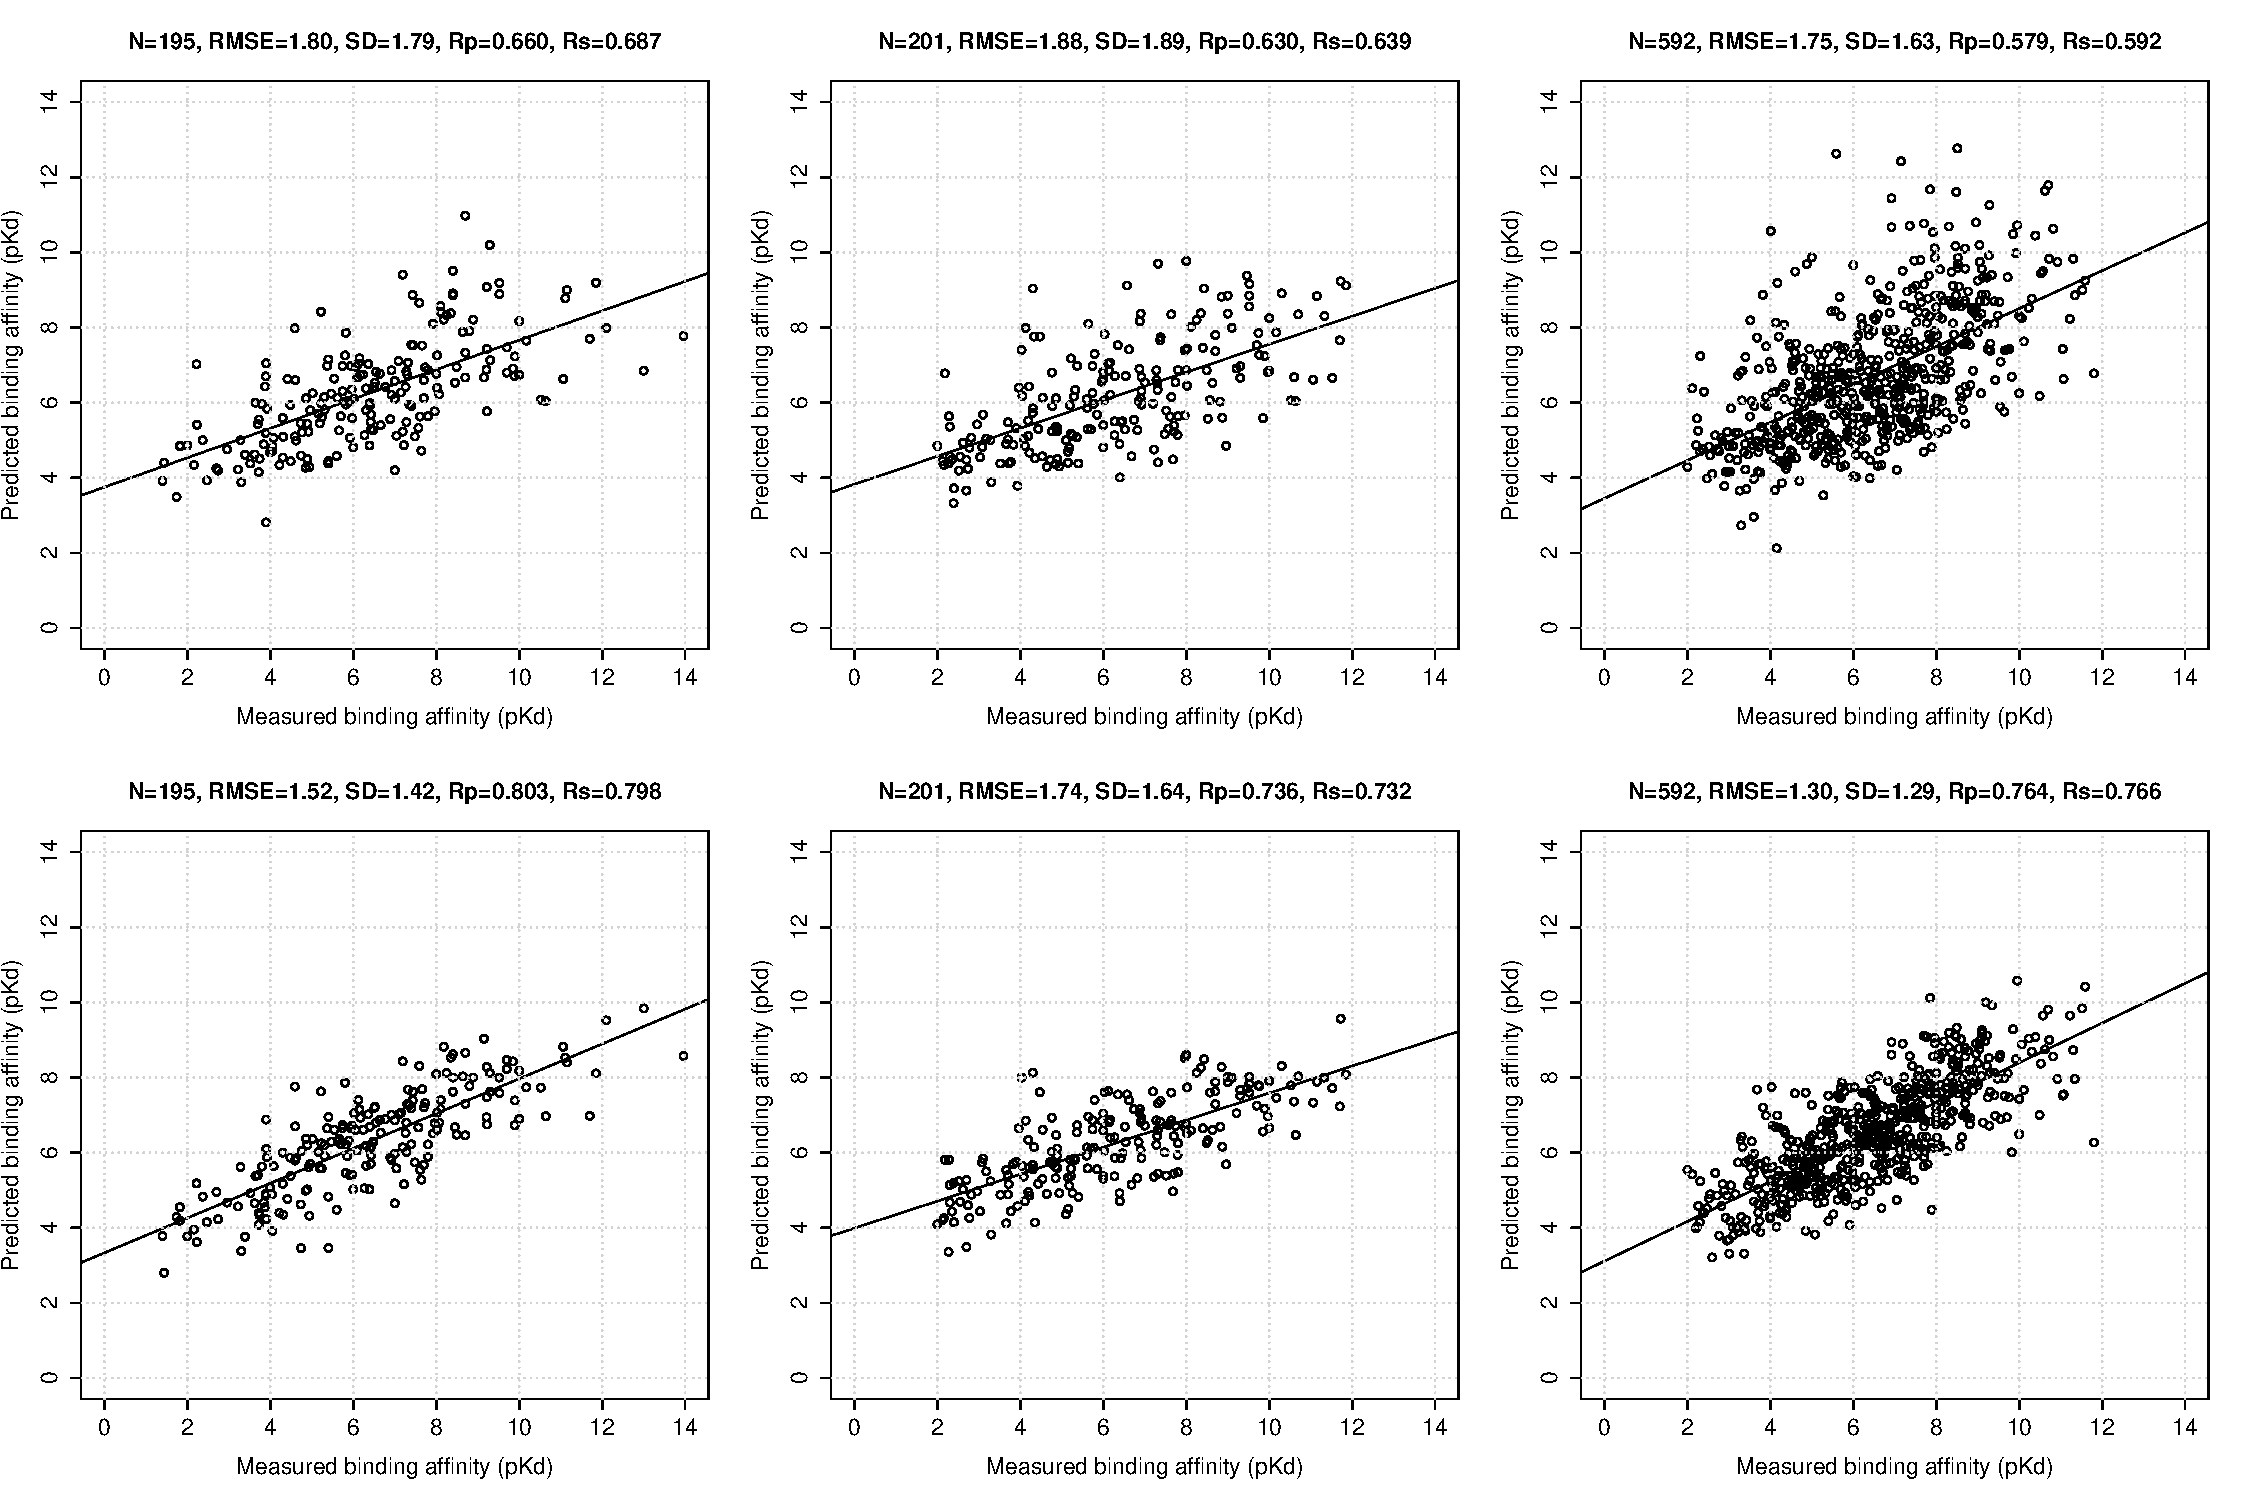
\includegraphics[width=\linewidth]{../rfcyscore/cor.pdf}
\caption{Correlation plots of predicted binding affinities against measured ones.}
\label{rfcyscore:cor}
\end{figure}

These results show that RF::CyscoreVinaElem performed consistently better than Cyscore on all the three benchmarks. It is important to note that, in each benchmark, both scoring functions used the same non-overlapping training and test sets. Taken together, these results suggest that one can develop a much more accurate scoring function out of an existing one simply by changing the regression model from MLR to RF and incorporating more structural features and training samples.

\subsection{Sensitivity analysis of the RF model can estimate feature importance}

RF-based scoring functions, unlike classical scoring functions, can barely be explicitly expressed as a mathematical equation like equation \eqref{rfcyscore:cyscore}. Therefore it is useful to employ the variable importance tool of RF to estimate the importance of each feature by randomly permuting its training values, and the feature leading to the largest variation in the predicted binding affinity on the OOB data can be regarded as the most important for a particular training set. Figure \ref{rfcyscore:varimp} plots the percentage of increase in mean square error (\%IncMSE) observed when each of the 4 Cyscore features used to train RF was noised up. The four features are hydrophobic free energy (Hydrophobic), van der Waals interaction energy (Vdw), hydrogen bond interaction energy (HBond) and ligand's conformational entropy (Ent). The \%IncMSE value of a particular feature was computed as the percentage of increase in mean square error observed in OOB prediction when that features was randomly permuted. All the 4 features turned out to be important (\%IncMSE\textgreater 20), with van der Waals interaction energy (Vdw) and hydrophobic free energy (Hydrophobic) being relatively more important (\%IncMSE\textgreater 40). Correctly estimating variable importance can assist in feature selection and in understanding ligand binding.

\begin{figure}
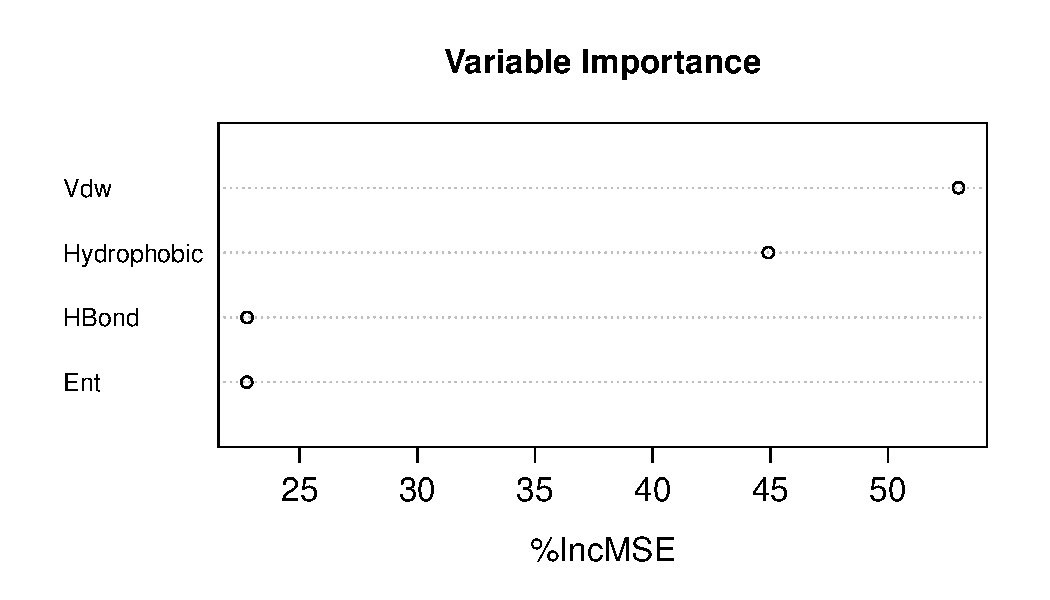
\includegraphics[width=\linewidth]{../rfcyscore/varimp.pdf}
\caption{RF::Cyscore feature importance estimated on internal OOB data of the 1105 complexes from PDBbind v2007 refined set.}
\label{rfcyscore:varimp}
\end{figure}

\section{Conclusions}

We have demonstrated that the multiple linear regression (MLR) model used in many scoring functions like Cyscore does not improve its performance in the presence of abundant training samples. This is a especially significant drawback for MLR-based scoring functions because they cannot benefit from the increasing availability of future experimental data. On the other hand, RF-based scoring functions can comprehensively capture the non-linear nature in the data and thus assimilate data significantly better than MLR-based scoring functions. Most importantly, feeding more training samples to RF can increase its predictive performance. Under this circumstance, improvements with dataset size can only be gained with the appropriate regression model. Changing the regression model of Cyscore from MLR to RF and expanding the feature set and the sample set can significantly increase the predictive accuracy. The performance gap between MLR-based and RF-based scoring functions will be further widened by the future availability of more and more X-ray crystal structures.

Classical empirical scoring functions typically rely on complicated energetic contributions that must be carefully devised from intermolecular interactions, whereas RF-based scoring functions can also effectively exploit features as simple as occurrence count of intermolecular contacts. It has also been shown in a previous study that functional group contributions in protein-ligand binding are non-additive. This means novel features can be difficult to be incorporated into an existing MLR model. In this study we have shown that using more structural features appropriately can also substantially boost the predictive accuracy of RF, as can be seen in the comparison between RF::CyscoreVinaElem and RF::Cyscore. This further stresses the importance of substituting RF for MLR in scoring function development.

\section{Future works}

The PHOENIX \citep{576} scoring function uses calorimetry data to decompose the change of binding free energy into change of enthalpy and change of entropy. It is an empirical scoring function that uses shape and volume descriptors to independently model enthalpic and entropic contributions. It is interesting to see how the predictive performance changes if RF is utilized for regression.

\chapterend
